\section{Experiments and Results}

We use measures of precision, recall, and F1 score for classifier assessment. In the binary confusion matrix, true positive (TP) indicates correct classification of data as some protocol class $C$. True negative (TN) is correct classification of data as \textit{not} class $C$. false negative (FN) implies incorrect identification of traffic as not $C$, and false positive (FP) is the incorrect classification of data as $C$.
\begin{equation}
\begin{split}
    R(C) = \frac{TP}{TP + FP} \text{,  }
    P(C) = \frac{TP}{TP + FN} \text{,  }
    F1(C) = \frac{2(P\times R)}{P + R} \\
    \end{split}
\end{equation}

A high recall indicates that in the binary problem, much of the traffic is correctly identified as the positive class. High precision in the model shows the quality of positive classifications, i.e. indicates how many were correctly classified out of everything said to be in the positive class. A model with low recall and high precision will likely mis-classify traffic which does belong in the positive class (high rate of false negatives), whereas a model with high recall and low precision will produce more false positives. In the following scenarios, we analyzed different potential traffic classification problems for port 443 based on the described attacks or opportunities from the threat models.

\subsection{VPN Traffic Profiling}

We analyzed the ISCX VPN/non-VPN dataset according to the applications and traffic types identified by the researchers who generated the data and Lotfollahi et al~\cite{deeppacket} who used the same data for per-packet classification in their Deep Packet models. They used a convolutional neural network and stacked autencoder model for implementations. We used three different configurations of \textsc{Forager} for the traffic and application classification tasks. For each problem, we ran a combination of \textsc{Alpine} and one of the payload transformation models. For application classification, DeepPacket's CNN model achieved very high F1 scores for most of the applications. Overall, each model is quite successful in distinguishing applications without inspecting packet contents, preserving user privacy while still accomplishing the mission. In the threat model, Alice could use our tool to better understand what kind of internet behavior Bob is engaging in over his VPN connection. We notice in both application and traffic classification tasks, our \textsc{Forager} models achieve some improved results in the VoIP categories. Our models also perform significantly better in profiling the benign/non-VPN traffic types, up to 0.13 higher than the stacked auto encoder in the VoIP category as well. When ICQ and AIM were combined under the Chat category, \textsc{Forager} achieves much higher results than any other model. For all models, distinguishing ICQ and AIM traffic was a difficult task. In further investigation into the network environment, we found both of these traffic streams were generated from the Pidgin messaging application, which makes sense that they were misclassified as one another in all the models. We also note that apps which use similar protocol stacks or likely similar APIs tend to be misclassified as one another. for example, FTPS and SFTP (both using FTP) are more difficult to distinguish from one another than either against SCP using SSH~\cite{deeppacket}. This is an important note for training and defining classes for neural network models in general, as well-defined classes or clusters make classification a clearer task. One significant difference in the experimental setup of Deep Packet versus \textsc{Forager} is that DeepPacket's CNN requires 300 epochs to train the entire network. \textsc{Maple} achieves near comparable results at a mere 10 epochs of training on the same data and split. \textsc{Date} also achieves good results only training with 10 epochs on its statistical model. We ran additional tests, increasing the number of epochs in order to determine if this improved our models' efficacy. In each case, 10 epochs proved to be sufficient for training \textsc{Forager} to maximum performance capability.

\begin{table*} [ht!]
\resizebox{\textwidth}{!}{\begin{tabular} {|p{2.3cm}|p{2.2cm}|p{2cm}|p{2cm}|p{2cm}|p{2cm}|}
\hline
\textbf{Application} & DeepPacket-CNN & DeepPacket-SAE & \textsc{Alpine} + \textsc{Palm} & \textsc{Alpine} + \textsc{Maple} & \textsc{Alpine} + \textsc{Date} \\
\hline
\end{tabular}}
\resizebox{\textwidth}{!}{\begin{tabular} {|p{2cm}|p{0.7cm}p{0.7cm}p{0.7cm}|p{0.7cm}p{0.7cm}p{0.7cm}|p{0.7cm}p{0.7cm}p{0.7cm}|p{0.7cm}p{0.7cm}p{0.7cm}|p{0.7cm}p{0.7cm}p{0.7cm}|}
\hline
& \textit{P} & \textit{R} & \textit{F1} & \textit{P} & \textit{R} & \textit{F1} & \textit{P} & \textit{R} & %
\textit{F1} & \textit{P} & \textit{R} & \textit{F1} & \textit{P} & \textit{R} & \textit{F1} \\
\hline
AIM chat & 0.87 & 0.76 & \textbf{0.81} & 0.76 & 0.64 & 0.70 & 0.80 & 0.55 & 0.65 & 0.80 & 0.57 & 0.67 & 0.67 & 0.69 & 0.68 \\
Email & 0.97 & 0.82 & 0.89 & 0.94 & 0.99 & \textbf{0.97} & 0.81 & 0.76 & 0.79 & 0.74 & 0.80 & 0.77 & 0.86 & 0.73 & 0.79 \\
Facebook & 0.96 & 0.95 & \textbf{0.96} & 0.94 & 0.95 & 0.95 & 0.96 & 0.90 & 0.93 & 0.97 & 0.91 & 0.94 & 0.98 & 0.90 & 0.94 \\
FTPS & 1.00 & 1.00 & \textbf{1.00} & 0.97 & 0.77 & 0.86 & 1.00 & 0.98 & 0.99 & 0.99 & 0.99 & 0.99 & 0.99 & 0.99 & 0.99 \\
Gmail & 0.97 & 0.95 & \textbf{0.96} & 0.93 & 0.94 & 0.94 & 0.96 & 0.87 & 0.91 & 0.94 & 0.90 & 0.92 & 0.95 & 0.90 & 0.92 \\
Hangouts & 0.96 & 0.98 & \textbf{0.97} & 0.94 & 0.99 & 0.97 & 0.98 & 0.89 & 0.93 & 0.96 & 0.91 & 0.94 & 0.96 & 0.91 & 0.94 \\
ICQ & 0.72 & 0.80 & \textbf{0.76} & 0.69 & 0.69 & 0.69 & 0.47 & 0.93 & 0.63 & 0.59 & 0.89 & 0.71 & 0.60 & 0.89 & 0.72 \\
Netflix & 1.00 & 1.00 & \textbf{1.00} & 1.00 & 1.00 & 1.00 & 0.99 & 0.98 & 0.99 & 0.99 & 0.99 & 0.99 & 0.99 & 0.99 & 0.99 \\
SCP & 0.97 & 0.99 & 0.98 & 1.00 & 1.00 & \textbf{1.00} & 0.98 & 0.91 & 0.94 & 0.98 & 0.92 & 0.95 & 0.97 & 0.91 & 0.94 \\
SFTP & 1.00 & 1.00 & \textbf{1.00} & 0.70 & 0.96 & 0.81 & 0.99 & 1.00 & 1.00 & 0.99 & 1.00 & 0.99 & 0.99 & 1.00 & 1.00 \\
Skype & 0.94 & 0.99 & 0.97 & 0.95 & 0.93 & 0.94 & 0.99 & 0.95 & \textbf{0.97} & 0.98 & 0.92 & 0.95 & 0.98 & 0.92 & 0.95 \\
Spotify & 0.98 & 0.98 & \textbf{0.98} & 0.98 & 0.98 & 0.98 & 0.99 & 0.92 & 0.95 & 0.99 & 0.95 & 0.97 & 0.99 & 0.95 & 0.97 \\
Torrent & 1.00 & 1.00 & \textbf{1.00} & 1.00 & 1.00 & 1.00 & 0.99 & 0.97 & 0.98 & 0.98 & 0.99 & 0.98 & 0.98 & 0.99 & 0.98 \\
VoipBuster & 0.99 & 1.00 & 0.99 & 0.99 & 0.99 & 0.99 & 1.00 & 0.98 & 0.99 & 1.00 & 0.98 & 0.99 & 1.00 & 0.99 & \textbf{0.99} \\
Vimeo & 0.99 & 0.99 & \textbf{0.99} & 0.99 & 0.98 & 0.98 & 0.99 & 0.98 & 0.99 & 0.97 & 0.98 & 0.99 & 0.98 & 0.98 & 0.98 \\
Youtube & 0.99 & 0.99 & \textbf{0.99} & 0.98 & 0.99 & 0.99 & 0.99 & 0.94 & 0.96 & 0.96 & 0.96 & 0.96 & 0.96 & 0.96 & 0.96 \\
\hline
\end{tabular}}
\resizebox{\textwidth}{!}{\begin{tabular} {|p{2cm}|p{2.3cm}|p{2.4cm}|p{2.3cm}|p{2.4cm}|p{2.3cm}|}
\hline
\textbf{Traffic Type} & DeepPacket-CNN & DeepPacket-SAE & \textsc{Alpine} + \textsc{Palm} & \textsc{Alpine} + \textsc{Maple} & \textsc{Alpine} + \textsc{Date} \\
\hline
\end{tabular}}
\resizebox{\textwidth}{!}{\begin{tabular} {|p{2cm}|p{0.7cm}p{0.7cm}p{0.7cm}|p{0.7cm}p{0.7cm}p{0.7cm}|p{0.7cm}p{0.7cm}p{0.7cm}|p{0.7cm}p{0.7cm}p{0.7cm}|p{0.7cm}p{0.7cm}p{0.7cm}|}
\hline
& \textit{P} & \textit{R} & \textit{F1} & \textit{P} & \textit{R} & \textit{F1} & \textit{P} & \textit{R} & %
\textit{F1} & \textit{P} & \textit{R} & \textit{F1} & \textit{P} & \textit{R} & \textit{F1} \\
\hline
Chat & 0.84 & 0.71 & 0.77 & 0.82 & 0.68 & 0.74 & 0.95 & 0.81 & \textbf{0.87} & 0.93 & 0.64 & 0.76 & 0.82 & 0.72 & 0.77 \\
Email & 0.96 & 0.87 & 0.91 & 0.97 & 0.93 & \textbf{0.95} & 0.76 & 0.99 & 0.86 & 0.71 & 0.74 & 0.73 & 0.75 & 0.67 & 0.71\\
File Transfer & 0.98 & 1.00 & \textbf{0.99} & 0.98 & 0.99 & \textbf{0.99} & 0.99 & 0.91 & 0.95 & 0.74 & 0.93 & 0.82 & 0.74 & 0.93 & 0.82 \\
Stream & 0.92 & 0.87 & 0.90 & 0.82 & 0.84 & 0.83 & 0.99 & 0.98 & \textbf{0.99} & 0.99 & 0.98 & \textbf{0.99} & 0.99 & 0.98 & \textbf{0.99} \\
VoIP & 0.63 & 0.88 & 0.74 & 0.64 & 0.90 & 0.75 & 0.99 & 0.95 & \textbf{0.97} & 0.99 & 0.94 & 0.96 & 0.99 & 0.95 & \textbf{0.97} \\
VPN: Chat & 0.98 & 0.98 & \textbf{0.98} & 0.95 & 0.94 & 0.94 & 0.96 & 0.95 & 0.96 & 0.96 & 0.98 & 0.97 & 0.96 & 0.97 & 0.97 \\
VPN: Transfer & 0.99 & 0.99 & \textbf{0.99} & 0.98 & 0.95 & 0.97 & 1.00 & 0.98 & \textbf{0.99} & 1.00 & 0.98 & \textbf{0.99} & 1.00 & 0.98 & \textbf{0.99} \\
VPN: Email & 0.99 & 0.98 & \textbf{0.99} & 0.97 & 0.93 & 0.95 & 1.00 & 0.98 & \textbf{0.99} & 0.99 & 0.98 & \textbf{0.99} & 0.97 & 0.99 & 0.98 \\
VPN: Stream & 1.00 & 1.00 & \textbf{1.00} & 0.99 & 0.99 & 0.99 & 0.99 & 0.99 & 0.99 & 0.99 & 0.99 & 0.99 & 0.99 & 0.80 & 0.89 \\
VPN: Torrent & 1.00 & 1.00 & \textbf{1.00} & 0.99 & 0.97 & 0.98 & 0.99 & 0.99 & 0.99 & 0.98 & 0.99 & 0.99 & 0.83 & 1.00 & 0.91 \\
VPN: VoIP & 0.99 & 1.00 & \textbf{1.00} & 0.99 & 1.00 & 0.99 & 1.00 & 0.98 & 0.99 & 0.99 & 0.98 & 0.99 & 0.99 & 0.98 & 0.99 \\
\hline
\end{tabular}}
\label{tab:vpnresults}
\caption{Results for classifying VPN data.}
\end{table*}

\subsection{Tor Traffic Profiling}

\begin{table*} [ht!]
\centering
\resizebox{\textwidth}{!}{\begin{tabular} {|p{2cm}|p{2.3cm}|p{2.4cm}|p{2.3cm}|p{2.4cm}|p{2.3cm}|}
\hline
\textbf{Application} & DeepPacket-CNN & DeepPacket-SAE & \textsc{Alpine} + \textsc{Palm} & \textsc{Alpine} + \textsc{Maple} & \textsc{Alpine} + \textsc{Date} \\
\hline
\end{tabular}}
\resizebox{\textwidth}{!}{\begin{tabular} {|p{2cm}|p{0.7cm}p{0.7cm}p{0.7cm}|p{0.7cm}p{0.7cm}p{0.7cm}|p{0.7cm}p{0.7cm}p{0.7cm}|p{0.7cm}p{0.7cm}p{0.7cm}|p{0.7cm}p{0.7cm}p{0.7cm}|}
\hline
& \textit{P} & \textit{R} & \textit{F1} & \textit{P} & \textit{R} & \textit{F1} & \textit{P} & \textit{R} & %
\textit{F1} & \textit{P} & \textit{R} & \textit{F1} & \textit{P} & \textit{R} & \textit{F1} \\
\hline
AIM chat & -- & -- & -- & -- & -- & -- & 0.86 & 0.53 & \textbf{0.66} & 0.95 & 0.50 & 0.65 & 0.96 & 0.49 & 0.65 \\
Chrome & 0.00 & 0.00 & 0.00 & 0.03 & 0.44 & 0.06 & 0.93 & 0.68 & 0.78 & 0.91 & 0.74 & 0.81 & 0.91 & 0.75 & \textbf{0.82}\\
Email & -- & -- & -- & -- & -- & -- & 0.94 & 0.84 & 0.89 & 0.94 & 0.85 & 0.89 & 0.94 & 0.85 & \textbf{0.90} \\
Facebook & 0.10 & 0.24 & 0.14 & 0.06 & 0.28 & 0.09 & 0.97 & 0.88 & 0.92 & 0.97 & 0.89 & \textbf{0.93} & 0.97 & 0.89 & \textbf{0.93} \\
FTPS & -- & -- & -- & -- & -- & -- & 0.95 & 0.99 & \textbf{0.97} & 0.95 & 0.99 & \textbf{0.97} & 0.95 & 0.99 & \textbf{0.97} \\
Gmail & 0.97 & 0.95 & 0.96 & 0.93 & 0.94 & 0.94 & 0.94 & 0.85 & 0.89 & 0.89 & 0.90 & 0.89 & 0.94 & 0.86 & \textbf{0.90} \\
Hangouts & -- & -- & -- & -- & -- & -- & 0.91 & 0.93 & \textbf{0.95} & 0.95 & 0.92 & 0.93 & 0.93 & 0.94 & 0.94 \\
ICQ & -- & -- & -- & -- & -- & -- & 0.40 & 0.94 & 0.56 & 0.51 & 0.97 & \textbf{0.67} & 0.48 & 0.98 & 0.65 \\
Netflix & -- & -- & -- & -- & -- & -- & 0.98 & 0.98 & 0.98 & 0.98 & 0.99 & 0.98 & 0.99 & 0.98 & \textbf{0.99} \\
SCP & 0.97 & 0.99 & 0.98 & 1.00 & 1.00 & 1.00 & 0.99 & 0.90 & 0.94 & 0.96 & 0.92 & 0.93 & 0.96 & 0.92 & \textbf{0.94} \\
SFTP & -- & -- & -- & -- & -- & -- & 1.00 & 0.94 & \textbf{0.97} & 0.99 & 0.94 & 0.97 & 0.99 & 0.94 & 0.97 \\
Skype & -- & -- & -- & -- & -- & -- & 0.97 & 0.91 & \textbf{0.94} & 0.95 & 0.92 & 0.93 & 0.96 & 0.91 & 0.93 \\
Spotify & -- & -- & -- & -- & -- & -- & 0.79 & 0.91 & \textbf{0.85} & 0.75 & 0.95 & 0.84 & 0.74 & 0.95 & 0.83 \\
VoipBuster & -- & -- & -- & -- & -- & -- & 1.00 & 0.98 & \textbf{0.99} & 1.00 & 0.98 & \textbf{0.99} & 1.00 & 0.98 & \textbf{0.99} \\
Vimeo & 0.44 & 0.36 & 0.40 & 0.05 & 0.91 & 0.09 & 0.98 & 0.94 & 0.96 & 0.95 & 0.95 & 0.95 & 0.97 & 0.95 & \textbf{0.96} \\
Vuze & -- & -- & -- & -- & -- & -- & 0.98 & 0.72 & 0.83 & 0.97 & 0.73 & \textbf{0.83} & 0.97 & 0.71 & 0.82 \\
Youtube & -- & -- & -- & -- & -- & -- & 0.95 & 0.94 & 0.94 & 0.94 & 0.95 & 0.95 & 0.94 & 0.96 & \textbf{0.95} \\
\hline
\end{tabular}}
\caption{Results for classifying Tor data by application.}
\label{tab:torappresults}
\end{table*}

\begin{table*}[h!]
\centering
\resizebox{\textwidth}{!}{\begin{tabular} {|p{2cm}|p{2.3cm}|p{2.3cm}|p{2.3cm}|p{2.4cm}|p{2.3cm}|}
\hline
\textbf{Traffic Type} & DIDarknet & J48 & \textsc{Alpine} + \textsc{Palm} & \textsc{Alpine} + \textsc{Maple} & \textsc{Alpine} + \textsc{Date} \\
\hline
\end{tabular}}
\resizebox{\textwidth}{!}{\begin{tabular} {|p{2cm}|p{0.7cm}p{0.7cm}p{0.7cm}|p{0.7cm}p{0.7cm}p{0.7cm}|p{0.7cm}p{0.7cm}p{0.7cm}|p{0.7cm}p{0.7cm}p{0.7cm}|p{0.7cm}p{0.7cm}p{0.7cm}|}
\hline
& \textit{P} & \textit{R} & \textit{F1} & \textit{P} & \textit{R} & \textit{F1} & \textit{P} & \textit{R} & \textit{F1} & \textit{P} & \textit{R} & %
\textit{F1} & \textit{P} & \textit{R} & \textit{F1} \\
\hline
Audio & 0.92 & 0.92 & 0.92 & 0.97 & 0.97 & \textbf{0.97} & 0.99 & 0.94 & 0.96 & 0.99 & 0.94 & 0.96 & 0.99 & 0.94 & 0.96 \\
Browsing & 0.55 & 0.47 & 0.51 & 0.99 & 0.99 & \textbf{0.99} & 0.97 & 0.94 & 0.95 & 0.95 & 0.97 & 0.96 & 0.95 & 0.97 & 0.96 \\
Chat & 0.90 & 0.86 & 0.88 & 0.93 & 0.93 & \textbf{0.93} & 0.92 & 0.74 & 0.82 & 0.84 & 0.80 & 0.82 & 0.93 & 0.70 & 0.80 \\
Email & 0.66 & 0.67 & 0.67 & 0.93 & 0.93 & \textbf{0.93} & 0.90 & 0.90 & 0.90 & 0.91 & 0.87 & 0.89 & 0.92 & 0.86 & 0.89 \\
File Transfer & 0.74 & 0.75 & 0.75 & 0.98 & 0.98 & \textbf{0.98} & 0.99 & 0.92 & 0.96 & 0.99 & 0.92 & 0.96 & 0.99 & 0.92 & 0.96 \\
P2P & 0.90 & 0.95 & 0.93 & 0.99 & 0.99 & \textbf{0.99} & 0.96 & 0.98 & 0.97 & 0.95 & 1.00 & 0.97 & 0.96 & 0.99 & 0.97 \\
Video & 0.82 & 0.88 & 0.85 & 0.98 & 0.98 & \textbf{0.98} & 0.99 & 0.97 & \textbf{0.98} & 0.98 & 0.98 & \textbf{0.98} & 0.98 & 0.98 & \textbf{0.98} \\
VOIP & 0.58 & 0.61 & 0.59 & 0.99 & 0.99 & \textbf{0.99} & 0.72 & 0.97 & 0.83 & 0.82 & 0.96 & 0.89 & 0.71 & 0.99 & 0.82 \\
\hline
\end{tabular}}
\label{tab:tortrafficresults}
\caption{Results for classifying Tor data by traffic type.}
\end{table*}

Another type of tunneled traffic we want to identify and profile on port 443 is anything running over Tor. We again ran our three configurations of the \textsc{Forager} toolkit against the Tor dataset. Deep Packet~\cite{deeppacket} also ran their SAE and CNN models against this data, but only report a portion of results. We provide a comparison against what they do report for completeness, and note that the \textsc{Forager} models are a dramatic improvement in terms of capability. Their model is unable to handle most of the application classes, whereas \textsc{Forager} can adapt to all applications and returns results as high as those in the VPN classification task. This result demonstrates the versatility of \textsc{Forager} compared to the state-of-the-art and current existing frameworks. Table~\ref{tab:torappresults} shows results of the application classification task. We also show comparative results of traffic type classification with work performed by Lashkari et al~\cite{didarknet} in their DIDarknet system which uses a two-dimensional convolutional neural network to characterize VPN and Tor traffic. It is important to note that unlike Deep Packet and \textsc{Forager} models, DIDarknet's CNN relies on flow-based features. Both we and Deep Packet prefer a stateless approach for best-effort, per-packet classification and use features of the individual packets themselves. Choorod et al~\cite{choorod2022tor} provide results of single packet classification of the Tor dataset using features extracted with Charcount from the Posit toolkit along with a decision tree-based algorithm called J48. This performed remarkably well on the traffic type classification task, and we also compare against their results. They marginally outperform the \textsc{Forager}  system; but both identified Tor traffic with a much greater accuracy and F1 score than the flow-based system. Choorod et al did not provide results for application-based identification, and it is unclear if their method would generalize to any other problems or has been attempted on any other data sets. The experiment results demonstrate that the system could be used to isolate Tor traffic on port 443, or any traffic stream. In the context of the threat model, Alice can determine if and when Bob is using Tor routing, which is useful for further track and trace. She also has a much greater insight into the traffic type and applications than other models previously gave, advancing the state of the art. A summarization is provided in Table~\ref{tab:classresults}.


\begin{table}
\centering
\begin{tabular}{| p{5cm} | c  c  c  c  c|}
\hline
 \textbf{Class Set} & \textbf{Accuracy} & \textbf{P} & \textbf{R} & \textbf{F1} & \textbf{$\kappa$} \\
 \hline
Tor & 0.99 & 0.99 & 0.99 & 0.99 & 0.99\\
VPN & 0.97 & 0.98 & 0.97 & 0.97 & 0.98 \\
Standard & 0.99 & 0.99 & 0.99 & 0.99 & 0.99\\
\hline
\end{tabular}

\begin{tabular}{| p{5cm} | c  c  c  c  c |}
\hline
 \textbf{Class Set} & \textbf{Accuracy} & \textbf{P} & \textbf{R} & \textbf{F1} & \textbf{$\kappa$} \\
 \hline
 \textbf{VPN/nonVPN} & 0.97 & 0.98 & 0.97 & 0.97 & 0.97 \\
 Traffic Type & 0.86 & 0.88 & 0.86 & 0.86 & 0.82 \\
 Application & 0.92 & 0.93 & 0.92 & 0.92 & 0.82 \\
 \hline
 \end{tabular}

\begin{tabular}{| p{5cm} | c  c  c  c  c |}
\hline
 \textbf{Class Set} & \textbf{Accuracy} & \textbf{P} & \textbf{R} & \textbf{F1} & \textbf{$\kappa$} \\
 \hline
 \textbf{Tor/nonTor} & 0.99 & 0.99 & 0.99 & 0.99 & 0.99 \\
 Traffic Type & 0.97 & 0.97 & 0.97 & 0.97 & 0.96 \\
 Application & 0.89 & 0.91 & 0.89 & 0.89 & 0.88 \\
 \hline
 \end{tabular}
\caption{Results for VPN/Tor classification}
\label{tab:classresults}
\end{table}

\subsection{Plaintext Traffic over HTTPS}
Our next experiment was to assess the ability of the model to determine if traffic samples on port 443 are truly encrypted packets (TLS) or not. Many firewalls are configured to default-allow port 443 traffic; an attacker may send any content or malware over this port in order to attempt to bypass a firewall. Senders wishing to bypass middlebox technology may send non-TLS data over port 443 to avoid detection. It is thus significant for surveillance and law enforcement operations to monitor traffic on port 443 for non-encrypted data which may be decipherable. IoT devices also can send unencrypted traffic over port 443~\cite{wood2017cleartext} which may contain some useful information. Alice finds it incredibly useful to capture all plaintext data where possible as it can contribute to the legal summation of a case. We created two classes of encrypted and non-encrypted traffic, performed random under-sampling, and ran the model, generating results in Figures~\ref{fig:tlsnontls}, \ref{fig:tlscomp}, and \ref{fig:comptype}. The model tends to overselect traffic as encrypted, and underselect traffic which is plaintext. This is not surprising due to the variety of features present in the single plaintext category, versus the lack of common features generally found or uncovered in the encrypted class. In this case, model design may not be well-suited to a binary classification problem because the class \textit{plaintext} is not well-defined. This tuning factor should be considered by users of the \textsc{Forager} system during the configuration process.

\subsection{Compressed Traffic over HTTPS}
Compressed versus encrypted traffic both tend to exhibit highly entropic behavior, with the data approaching uniform distribution in more advanced implementations~\cite{hedge}. An attacker may run compressed data over port 443 (or any port) and middleware technology may assume it is encrypted if using statistical tests like Chi-squared or Shannon entropy~\cite{gaspari2020encod}. Instead, Alice could use our system to isolate compressed traffic from encrypted traffic, and thus be able to decompress and process that information in follow-on applications. In order to run this experiment, we first ran compression algorithms on the payloads of FTP\_DATA packets. We chose this traffic type as the payloads are largely text-based and often sent compressed over the wire. We used three standard compression libraries - \texttt{gzip}, \texttt{zlib}, and \texttt{bz2}. The packets were randomly divided into groups, producing 10,519 sample compressed payloads of each type. The encrypted traffic from the ISCX 2016 VPN-nonVPN dataset~\cite{iscx-vpn-paper} was used for the encrypted traffic type. Figure~\ref{fig:tlscomp} shows \textsc{Forager} is capable of identifying compressed from encrypted traffic on port 443 or out of any stream (using \textsc{Alpine} and \textsc{Maple}). Furthermore, we can profile down to specific compression type with great accuracy in Figure~\ref{fig:comptype}. We can also identify plaintext traffic in Figure~\ref{fig:tlsnontls}. Alice could use this technology to extract compressed data streams and decompress them for further analysis.

\begin{figure} [ht!]
\centering
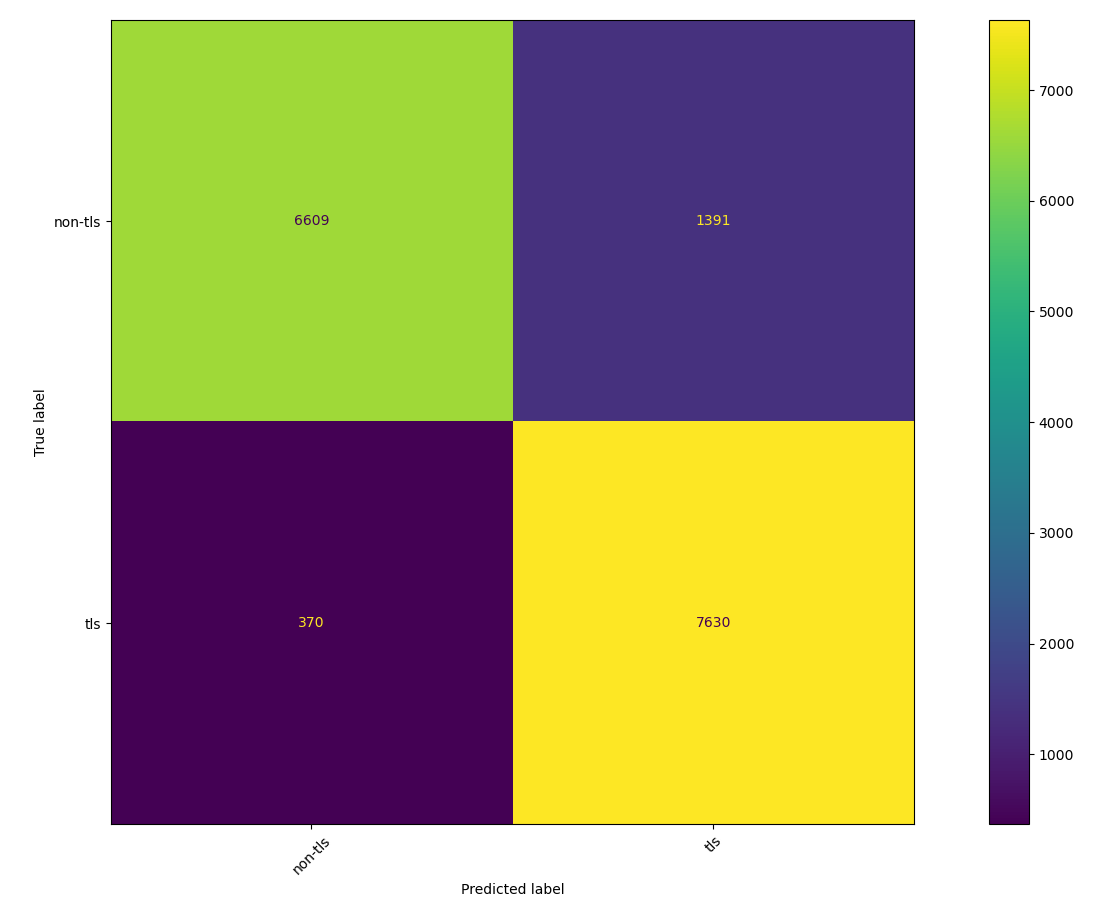
\includegraphics[scale=0.4]{chapters/7/img/tls_nontls.png}
\caption{Plaintext versus encrypted traffic results.}
\label{fig:tlsnontls}
\end{figure}

\begin{figure} [ht!]
\centering
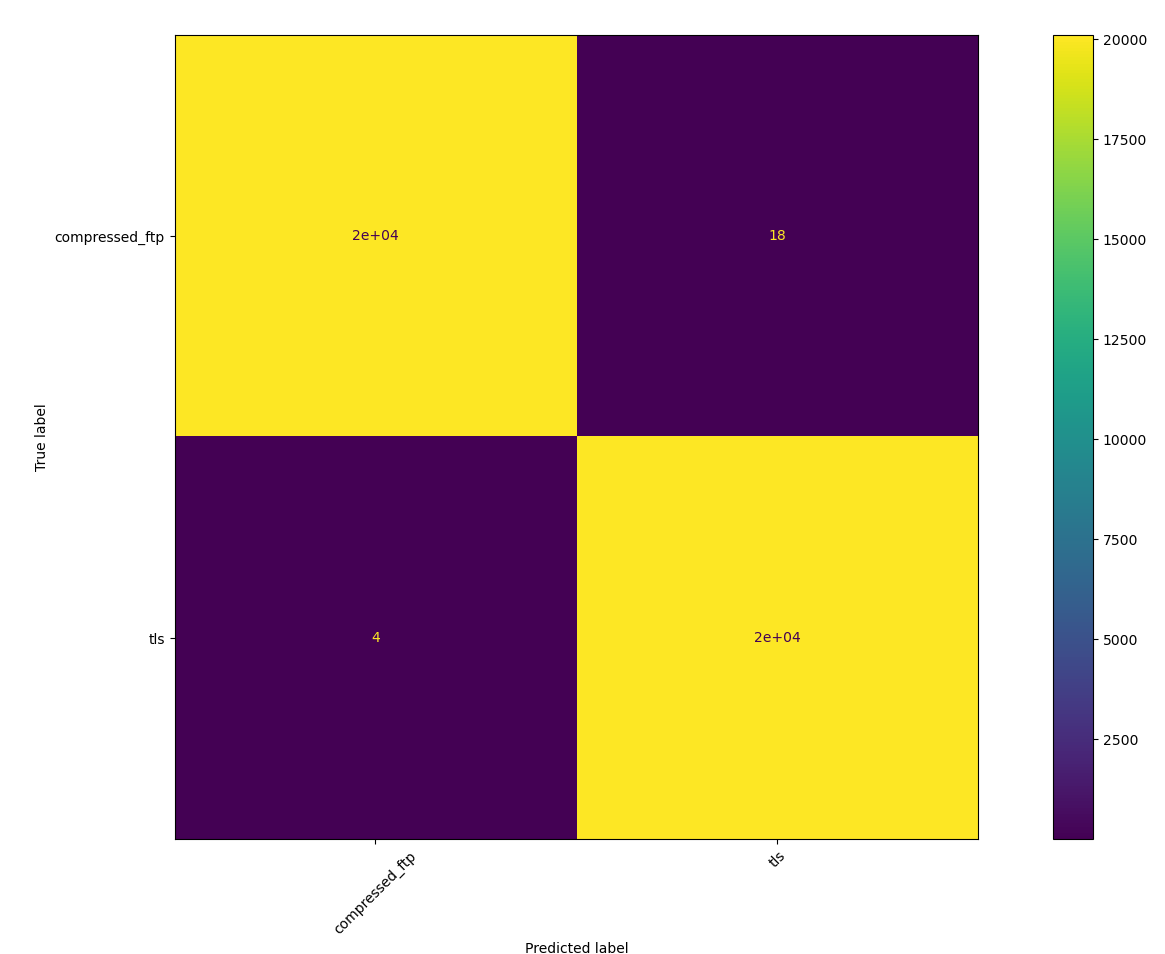
\includegraphics[scale=0.4]{chapters/7/img/compressed_tls.png}
\caption{Compressed versus encrypted traffic results.}
\label{fig:tlscomp}
\end{figure}

\begin{figure} [ht!]
\centering
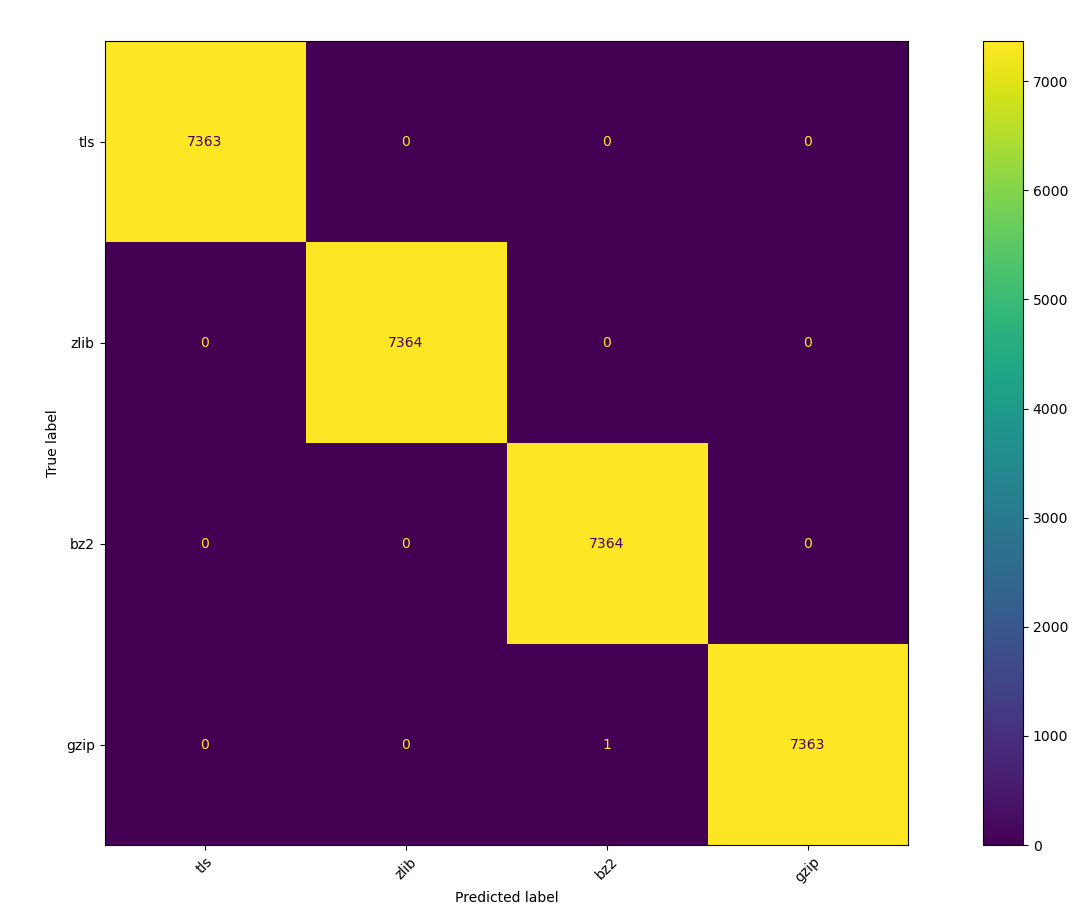
\includegraphics[scale=0.4]{chapters/7/img/encrypted_compressed.png}
\caption{Compressed versus encrypted traffic results.}
\label{fig:comptype}
\end{figure}


\begin{table}
\centering
\begin{tabular}{| c | p{0.6cm}  p{0.6cm}  p{0.6cm} |}
 \hline
 \textbf{Protocol} & \textbf{P} & \textbf{R} & \textbf{F1}\\
 \hline
 Encrypted & 1.00 & 1.00 & 1.00\\
 Compressed & 1.00 & 1.00 & 1.00\\
 \hline
 Encrypted & 0.85 & 0.95 & 0.90\\
 Plaintext & 0.95 & 0.83 & 0.88\\
 \hline
 TLS & 1.00 & 1.00 & 1.00\\
 BZ2 & 1.00 & 1.00 & 1.00\\
 GZIP & 1.00 & 1.00 & 1.00\\
 ZLIB & 1.00 & 1.00 & 1.00\\
 \hline
\end{tabular}
\caption{Results for encryption and compression detection}
\end{table}

\subsection{SSH over HTTPS}
We want to be able to identify particular instances of certain protocols over an encrypted traffic network; One such protocol of interest is SSH. This is often used to bypass firewall restrictions or create covert data channels. In our experiments, we implemented the same model combinations as with the previous scenarios. The \textsc{Forager} toolkit was highly successful in classifying SSH traffic from the SSH-over-HTTPS dataset generated by the EMews simulator, achieving over 99\% accuracy as shown in Table~\ref{tab:dohsohresults}. Identifying this traffic would allow inspectors to both mitigate covert data channels or monitor them for possible illicit activity. For example, Alice could detect any open covert data channels Bob might attempt to create over SSH.

\subsection{DNS over HTTPS}
Our final experiment was to detect DNS traffic running over HTTPS. A perpetual challenge for security research in classification and anomaly detection is the notion of intent; just because something is identified as belonging to a particular class or marked as an outlier does not always correlate that it is malicious. For example, a new instance of a running process can just be that - a user running a new program - and not necessarily an executing malware. Or a malformed data packet may appear different than others in the stream, but that could just be a bad transmission. For DNS over HTTPS, mainstream browsers like Chrome and Firefox employ this technique without malicious intent. As such, being able to determine DNS tunneling as a second layer to the DoH/non-DoH identification is of critical importance.
 The results in Table~\ref{tab:dohsohresults} show that \textsc{Forager} rises to meet this challenge, and can distinguish both DoH/non-DoH traffic and then malicious traffic from the identified DoH traffic with high accuracy and few false positives. Thus, any attempt Bob makes at DoH tunneling is now detectable using our toolkit.

\begin{table} [ht!]
\centering
\begin{tabular} {|p{2.5cm}|p{2.5cm}|p{2.5cm}|p{2.5cm}|}
\hline
\textbf{Model} & A+P & A+M & A+D \\
\hline
\end{tabular}
\begin{tabular} {|p{2cm}|p{0.6cm}p{0.6cm}p{0.6cm}|p{0.6cm}p{0.6cm}p{0.6cm}|p{0.6cm}p{0.6cm}p{0.6cm}|}
\hline
\textbf{Class} & \textit{P} & \textit{R} & \textit{F1} & \textit{P} & \textit{R} & \textit{F1} & \textit{P} & \textit{R} & \textit{F1} \\
\hline
\hline
\textit{SSH} & 1.00 & 0.99 & 1.00 & 0.98 & 1.00 & 0.99 & 1.00 & 1.00 & 1.00 \\
\textit{Non-SSH} & 0.99 & 1.00 & 1.00 & 1.00 & 0.98 & 0.99 & 1.00 & 1.00 & 1.00 \\
\hline
\hline
\textit{DNS} & 1.00 & 0.97 & 0.98 & 0.96 & 0.99 & 0.98 & 0.95 & 0.99 & 0.97 \\
\textit{Non-DNS} & 0.97 & 1.00 & 0.98 & 0.99 & 0.96 & 0.97 & 0.95 & 0.97 & 0.96 \\
\hline
\hline
\textit{Malicous} & 1.00 & 0.95 & 0.97 & 1.00 & 0.95 & 0.97 & 0.99 & 0.95 & 0.97 \\
\textit{Benign} & 0.96 & 1.00 & 0.98 & 0.95 & 1.00 & 0.97 & 0.96 & 0.99 & 0.97 \\
\hline
\end{tabular}
\caption{Results for classifying DoH/non-DoH and SoH/non-SoH data.}
\label{tab:dohsohresults}
\end{table}

\subsection{Performance Metrics}

The experiments were run on a 1.6 GHz Dual-Core Intel Core i5 processor with 16GB of RAM running MacOS Big Sur version 11.6.1. For each of our experiments, we tracked system performance metrics for the models as they performed the classification task and provide this data in Appendix A. This is important for real systems to assess not only the expected tonnage of network traffic they can process, but also to determine what models may be appropriate for deployment. For example, a model whose strategy focuses on online training may not be suitable in an environment who requires high throughput and low downtime, but has a high training time. Or, in some scenarios it may be acceptable to have slightly lower accuracy but a higher throughput rate.
